\documentclass[11pt,oneside,a4paper]{article}
\usepackage[table]{xcolor}
\usepackage{graphicx}
\usepackage{fancyhdr}
\usepackage{hyperref}
\pagestyle{fancy}
\lfoot{Louis-Joseph AMAS}
\cfoot{\thepage}
\renewcommand*\contentsname{Sommaire}

\begin{document}

\title{More Flexible Smart Contract Languages for Permissioned
Blockchains and Distributed Ledgers}
\author{Louis-Joseph AMAS}
\date{16 décembre 2020}
\maketitle

\begin{center}
  
\includegraphics[scale=0.5]{polytech.jpg}
\end{center}

\begin{center}
  
\includegraphics[scale=0.5]{inria.jpg}
\end{center}

\begin{abstract}
Ce rapport présente mon projet de fin d'études mené à l'Inria Sophia Antipolis-Méditerranée. 
Le projet consista à explorer le fonctionnement des Smart Contract. L'objectif a été de rechercher des moyens de rendre
les smarts contracts (qui par définition son non immuable) modifiable.
Plus en détails, j'ai dû concevoir la mise en place de prototype (PoC: Proof of concept) démontrant la possibilité de modification,
de plus, j'ai dû comprendre les problèmes soulevés par cette nouvelle liberté et proposé de solutions.
Dans le cadre de ce projet, j'ai pu travailler avec Mr Luigi Liquori, Mr Daniel de Carvalho et Mr Mansur Khazeev dans le cadre de multiples réunions. 
J'ai pu réaliser trois présentations oral sur ce sujet afin d'aider Mr Khazeev à réaliser sa thèse.

\end{abstract}
\newpage
\tableofcontents

\newpage
\section{Introduction}

Statut: Terminé

Tout d’abord, il est nécessaire d’expliquer le concept des technologies concernées. La
blockchain est une technologie permettant de faire la représentation d’un registre de compte de
manière numérique et distribué. Cela permet de s’affranchir d’un tiers de confiance, la première
technologie réalisant ces objectifs est le Bitcoin. 

Le Bitcoin est une monnaie décentralisée basé sur
la blockchain. C'est un registre de compte contenant toutes les transactions effectuées. Pour sécuriser
les accès à ce registre (permettre au ayant droit d’un compte de dépenser son argent), Bitcoin
combine deux principes fondamentaux, la cryptographie à clé publique ainsi que la signature
numérique, La cryptographie à clé publique permet de vérifier que un utilisateur possède réellement
un compte. La signature numérique permet de vérifier l’intégrité des transactions. Les transactions
sont des éléments d’un bloc et les blocs sont chaînés (mis les uns après les autres) à l’aide de la
signature numérique. Ce principe de chaîne permet d’assurer que si l’une des transactions est
modifiée alors la signature est modifiée. Une personne malveillante modifiant une transaction déjà
inscrite dans la chaîne de bloc sera détectée.

Des améliorations à ce principe de blockchain on était faite et il existe maintenant une
technologie appelée "smart contract". Cette technologie est un moyen d’exécuter un programme
de manière distribuée, permettant de s’affranchir d’un tiers de confiance. Cela peut être utilisé pour
réaliser par exemple des systèmes de vote sans possibilité de triche ou de modification du résultat
ou bien représenter un jeu d’argent (poker, paris sportif...). Cette technologie est enregistrée de la
même manière dans un registre non modifiable. L’ojectif de ce projet et de rechercher les manières
de pouvoir modifier le programme exécuter par un smart contract afin d’adapter le comportement
dynamiquement selon les besoins.


\newpage
\section{Contexte technologique}

\subsection{Blockchain}

\subsubsection{Bitcoin}

Une (ou un) blockchain, ou chaîne de blocs.  Techniquement, il s'agit d'une base de données distribuée dont les informations stockées sont vérifiées 
et groupées à intervalles de temps réguliers sous forme de bloc, formant ainsi une chaîne de blocs. L'ensemble est sécurisé par cryptographie. 
La chaîne de blocs est alors stocké sur de multiple machine en même temps que l'on appelle des nœuds. 
Cette chaîne permet de protéger contre la falsification et la modification de la base de données par les nœuds de stockage.
C'est donc un registre distribué et sécurisé de toutes les transactions effectuées depuis le démarrage du système réparti.

La première technologie déployant un tel système est le Bitcoin. Le Bitcoin utilise la blockchain afin de représenter un registre de compte
distribué. Les utilisateurs souhaitant utiliser cette cryptomonnaie génère une paire de clé asymétrique.

Pour rappel, les chiffrements asymétriques sont constitués de deux clés l'une publique disponible par tous le monde et l'une privée qui doit
rester secrète. Les méthodes de chiffrements à clé publique permettent e de rendre un message inintelligible par toute personne n'ayant pas la clé 
privée d'un message chiffré par la clé publique complémentaire. Cette technique de chiffrement permet aussi de vérifier (Signer numériquement) qu'un
message a bien été écrit par quelqu'un possédant une paire de clé (Privée, publique).

Bitcoin utilise cette fonctionnalité afin d'autoriser une personne à échanger son argent. Un bloc de la blockchain Bitcoin contient des transactions
(des échanges de jeton BTC) signer par la clé privée de l'utilisateur souhaitant transférer ses jetons. Bitcoin calcul le hash de toutes ses 
transactions et crée un bloc à l'aide de la concaténation de tous les hashs de toutes les transactions ainsi que le hash du bloc précédent.

Cela permet de rendre quasi impossible la falsification et la modification de la chaîne. En effet, un attaquant voulant modifier la chaîne serait
détecté car, le hash de son bloc serait invalide s'il modifie même qu'une transaction. Le Bitcoin réalise l'exploit de créer un équivalent a l'argent
liquide mais numériquement.

\subsubsection{Ethereum}

Ethereum est une technologie qui révolutionne la blockchain en y ajoutant une fonctionnalité très intéressante nommé les smarts contract. Cette
technologie est toujours basée sur le même principe que Bitcoin afin de valider ses transactions mais ajoute quelques nouvelles fonctionnalités.

\subsection{Smart contract}

Les contrats intelligents ou smart contracts sont des protocoles permettant d'exécuter du code de manière distribuée dans un environnement blockchain.
Ce mécanisme permet de s'affranchir de l'architecture client / serveur mais aussi, des architectures distribuées traditionnels. Les développeurs de
tel smart contract peuvent assumer que leurs contract une fois déployé sur la blockchain est immuable et décentralisé.

L'immuabilité de tel contrat permet de gagner la confiance des utilisateurs. Un utilisateur peut regarder le code du contrat déployé est être sûr 
de son comportement. Cela permet par exemple de programmer des jeux d'argents de manière numérique sans tierce de confiance mathématiquement 
vérifiable juste.

\subsubsection{Smart contract modifiable}
Un contrat auto modifiable est un contrat qui à la capacité suite à la réception ou à la
comparaison de données de se modifier seul. En effet, un contrat peut avoir besoin de
modifier son comportement quand certaines conditions sont respectées.

\subsubsection{EVM}

Pour créer une tel technologie Ethereum utilise l'Ethereum Virtual Machine (EVM) cette machine virtuelle peut être comparé à la JVM mais de manière distribuée.
L'EVM est une machine basée sur une \emph{pile distribuée sur réseaux}.
L'EVM est exécutée sur chaque nœud du réseau Ethereum. Et chaque exécution est signé de la même manière que Bitcoin afin de protéger contre la falsification
ou la modification d'une exécution.

\subsubsection{Solidity}

Solidity est un langage de programmation orienté objet dédié à l'écriture de contrats intelligents. Il est utilisé pour implémenter des smarts contrat sur diverses 
blockchains, notamment Ethereum. Solidity est un langage inspiré des langages orientées objets et plus en particulier du langage Javascript. L'objectif de ce stage est de rendre simple et
compréhensible le développement de smart contracts à tous. Néanmoins sa simplicité peut causer des problèmes car, il n'y a pas de moyen simple de vérifier (à la différence d'un langage fonctionnel)
l'exactitude du programme.  Sachant que les smarts contracts représentent souvent de l'argent il est très important de faire attention au code déployé.


\newpage
\section{Mes Objectifs et les scénarios}

\subsection{Objectifs}

Les objectifs de ce projet ont été les suivants et inspirés au papier scientifique \cite{OOPSLA} qui évoquait un langages de programmation object-based où les méthodes se pouvaient modifier (de façon sûre) par un simple appel de méthode (\emph{self-inflicted extension}):

\begin{itemize}
    \item Créer un prototype de modèle de smart contract modifiable.
    \item Comparaison de ma solution avec une bibliothèque populaire.
    \item Comparaison avec l'état de l'art standard.
\end{itemize}

Dès débuts du mois d'octobre, j'ai commencé à me renseigner sur les technologies présentées au chapitre
précédent. Suite à quelque réunion avec Mr. Luigi Liquori, Directeur de Recherche Inria, nous avions trouvé un chemin vers lequel je pouvais m'orienter afin de réaliser mon premier \emph{smart contract modifiable}.

Nous avons alors pris la décision de réaliser des prototypes intégralement par nous même.
L'objectif est ici d'apprendre les bases du développement et déploiement d'un tel contrat,
sans profiter d'aucune abstraction.

Une fois ce prototype terminé nous avions prévu de comparer cette solution a l'implémentation
de la bibliothèque \emph{OpenZeppelin} \cite{OpenZeppelin}. Cette bibliothèque étant l'un des standard de l'environnement
des smarts contract Ethereum.

Durant le mois de projet, j'ai aussi contacté l'équipe de développeurs d'Ethereum afin d'obtenir
des ressources sur le sujet. Cette équipe m'a répondu est m'a envoyé les dernières techniques du
domaine. Nous avons alors décidé d'ajouter comme objectif la comparaison avec des techniques les
plus avancés avec mon prototype et l'implémentation d'OpenZeppelin.

\subsection{Scénarios et \emph{Use Cases}}

\subsubsection{Scénario 1}

Un état souhaite passer au vote électronique, il décide d’utiliser les smart contrats afin de
décentraliser leur solution. L’objectif est de prouver aux électeurs que le vote n’est pas truqué. L’état va
alors payer une équipe d’ingénieur afin de faire un système de vote qui pourra durer dans le temps.
Néanmoins ils souhaitent aussi pouvoir modifier le mécanisme de vote au fur des années. C’est ici que
mon projet de recherche prend tout son sens, je conseille cet état fictif d’utiliser mes recherches afin
d’utiliser un smart contract modifiable. L’objectif est pouvoir changer le système de vote dans le futur
tout en utilisant la technologie blockchain.

\subsubsection{Scénario 2}

Deux entreprises (A et B) souhaitent passer un accord, elles décident de partager leurs services
de ressources humaines pour réduire les frais. Elles décident de stocker le nombre d’heures passés à
travailler pour une entreprise de façon décentralisée (Smart Contract). Avec cette solution l’entreprise B
pourra être sûre que l’entreprise A ne ment pas et vice-versa. De plus A aimerait ajouter une nouvelle
entreprise dans quelques années au système. 
Pour cela, le smart contract doit pouvoir être modifié pour ne pas forcer A et
B de déployer un nouveau contrat contenant C (la nouvelle entreprise).


\newpage
\section{Prototypes}

Tous le code présenté ICI est accessible ici:
https://github.com/Louis-Amas/Projet\_TER

\begin{itemize}
    \item Phase de recherche.
    \item Comparaison avec une bibliothèque populaire.
    \item Comparaison avec le standard.
\end{itemize}

\subsection{Phase de recherche}

Pendant la phase de préparation du projet, je me suis renseigné sur toutes les manières de rendre un smart contract modifiable.
Mon temps de projet étant assez court, je me suis concentré sur une méthode nommée Proxy. Cette méthode permet de créer un
smart contract en façade qui déléguera les appels à un autre smart contract dit d'implémentation. J'ai aussi contacté
l'équipe de développement d'Ethereum afin d'obtenir plus de ressources. L'équipe de développement m'a répondu avec un document
contenant un récapitulatif de l'état de l'art sur la modification des smarts contracts. Une aubaine pour moi.

Ce document contenait de nombreux lien vers des répertoires Git, après quelques heures à lire le code source de ces répertoires,
et avec mes recherches en amont j'avais toutes les clefs nécessaires pour commencer. 

\subsection{Les outils}

Il me fallait un environnement de développement afin de commencer à programmer un prototype. L'Ethereum étant une technologie
décentralisée contenant plusieurs nœuds il est nécessaire d'utiliser des outils de simulation ou des réseaux de tests (Testnet).
J'ai opté pour la simulation de la blockchain Ethereum. J'ai utilisé la suite d'outil Truffle.

Truffle contient un logiciel permettant d'émuler une blockchain Ethereum mais aussi, des bibliothèques pour gérer tout le cycle 
de vie des smarts contracts, développement, compilation, déploiement et test.

Truffle se présente sous la forme d'une interface de commande et d'une architecture de fichier spécifique. Truffle m'a été très
utile pour tester mes smarts contracts. En effet, il est possible d'écrire des tests automatiques en Javascript afin
de vérifier le bon fonctionnement des smarts contract.

Truffle peut aussi être connecté à une vraie blockchain et donc être utilisé en production. De plus, quelqu'un voulant comprendre
ou réutiliser mon code, pourra exécuter mon code une fois qu'il aura configuré la blockchain sur laquelle déployé. Cela permet 
de simplifier l'environnement de développement. Durant ma phase
de recherche j'ai lu les tests Truffle des implémentations trouvés sur internet afin de mieux comprendre leurs fonctionnements.

L'outil Ganache est aussi très utile pour débuger les smarts contracts car, il est possible de lire chaque transaction et chaque
bloc de la blockchain simulé.

\subsection{Premier prototype}

Une fois tout en place j'ai pu commencer mon développement. J'ai décidé de commencer par l'implémentation d'un système de vote 
électronique comme décrit dans le scénario 1. J'ai programmé un système de vote simple permettant au créateur du vote de donner
le droit de voter a qu'il souhaite. Chaque utilisateur ayant le droit de vote peut alors voter pour un des candidats proposer par
le créateur du contrat. Je veux pouvoir avoir la possibilité de donner mon vote à quelqu'un d'autre, c'est-à-dire faire une 
procuration. Je souhaiterais pouvoir ajouter ou enlever dynamiquement cette fonctionnalité.

\subsubsection{Méthode utilisée}

Mon premier prototype réalise donc cette fonctionnalité. Pour réaliser cette modification alors que je rappelle 
qu'elle est normalement impossible car, les contrats sont immuable. J'ai utilisé une méthode appelée Proxy.
Pour cela, j'ai créé un contrat avec quelque particularité. J'ai utilisé la fonction "fallback()" de Solidity.
Cette fonction est appelée quand la fonction appelée sur un contrat n'existe pas. Cette fonctionnalité m'est très
utile, car je vais pouvoir à l'aide de l'opcode delegatecall transmettre touts les appels fait au contrat Proxy
au contrat contenant l'implémentation.

\begin{figure}
  \caption{Exemple de la méthode Proxy}
  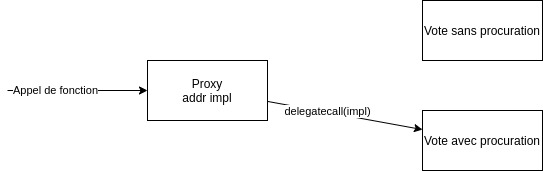
\includegraphics[scale=0.6]{proxy.jpg}
  \centering 
  \label{fig:proxy}
\end{figure}

\subsubsection{Détail technique}
L'opcode delegatecall permet d'exécuter du code se situant dans un autre contrat voir \pageref{fig:proxy}. 
Il prend en paramètre une adresse d'un autre contrat.

Néanmoins, il est important de bien comprendre comment Solidity stocke les variables dans un contract, afin de 
comprendre comment le code exécuter dans le contrat appelé par "delegatecall", peut-il interagir avec les variables.

En effet, l'opcode "delegatecall" à un comportement peu intuitif, delegatecall exécute le code d'un autre contrat
mais garde le stockage du contrat appelant "delegatecall". Cela veut dire que le contrat implémentation doit savoir comment 
les variables du contrat appelant sont stockées.

Solidity stocke les variables les une après les autres ($\forall n \in N, var_1 \mapsto pos_1, var_2 \mapsto pos_2,
..., var_n \mapsto pos_n$)

Pour la réalisation d'un contrat Proxy il est nécessaire d'avoir une variable contenant l'adresse d'une implémentation,
il est très important que le contrat contenant l'implémentation n'override pas son adresse.

Il existe deux méthodes pour s'assurer que cela n'arrive pas. La méthode la plus simple et de mettre la variable contenant
l'implémentation dans chaque contrat. 

\begin{figure}[h!]
  \caption{Exemple de la méthode Proxy avec stockage structuré}
  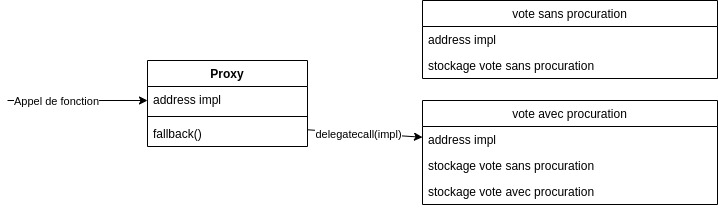
\includegraphics[scale=0.5]{proxy_structured_stockage.jpg}
  \centering 
  \label{fig:proxy_structuré}
\end{figure}

La deuxième méthode appelé stockage non structuré est de stocker l'adresse de l'implémentation à une position "aléatoire".
Pour cela, on peut placer la variable à la position retournée par le calcul de la fonction sha3 sur le nom de la variable.
La fonction sha3 étant une fonction de hash il y a très peu de risque de collision.

La méthode avec un stockage non structuré est une meilleure solution car, elle permet d'utiliser des contrats d'implémentation 
qui ne connaisse pas l'existence du Proxy.

\begin{figure}[h!]
  \caption{Exemple de la méthode Proxy avec stockage non structuré}
  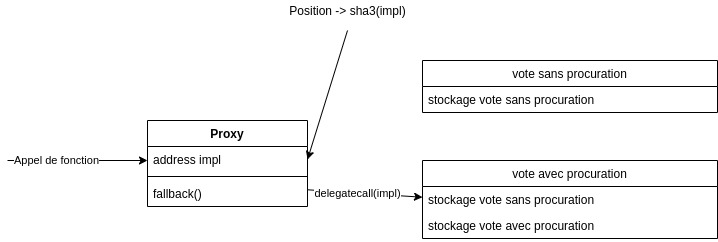
\includegraphics[scale=0.5]{proxy_unstructured.jpg}
  \centering 
  \label{fig:proxy_structuré}
\end{figure}

\subsection{Implémentation officielle (Diamond)}

En poursuivant mes recherches sur l'état de l'art du domaine j'ai trouvé sur le site internet des 
"Ethereum Improvement Proposals"(EIP). La proposition 2535 du 22 février 2020 ayant pour but de formaliser
la manière dont programmer un Proxy intelligent. Le principe sous-jacent est identique à mon prototype
avec un stockage non structuré mais, cette proposition y ajoute une interface plus simple et plus modulable.

En effet, l'objectif est de créer une bibliothèque avec une interface simple afin de permettre facilement à un
utilisateur de programmer son propre proxy personnaliser.

Ce diamant fonctionne de la manière suivante.

Un diamant est composé de facette chaque facette représente une fonction. Chaque facette permet de lier l'identificateur
de fonction à l'adresse d'un autre contrat. Quand un appel de fonction est exécuté sur un diamant alors celui-ci ira chercher
dans sa structure de données la facette correspondante à l'appel de fonction. Une fois cette facette trouvée il pourra alors
appeler delegatecall sur l'adresse associé à cette facette afin d'exécuter le coder situé dans un autre contract.

Afin d'ajouter, modifier ou supprimer une facette la bibliothèque proposée contient une fonction nommée "diamondCut".
Cette fonction prend en paramètre un tableau de "coupe de diamant". Une coupe de diamant est une structure contenant
une action (Ajouter, modifier ou supprimer), une adresse d'un contract et un tableau de sélecteur de fonction. Voir la figure
\pageref{fig:diamond_struct}

Un développeur voulant utiliser cette bibliothèque aura juste à générer un tableau de "coupe de diamant" modélisant le 
proxy qu'il souhaite réaliser. La seule obligation du développeur est d'utiliser uniquement un stockage non structuré dans
ces facettes.

\begin{figure}[h]
  \caption{Schéma représentatif du fonctionnement internet d'un diamant.}
  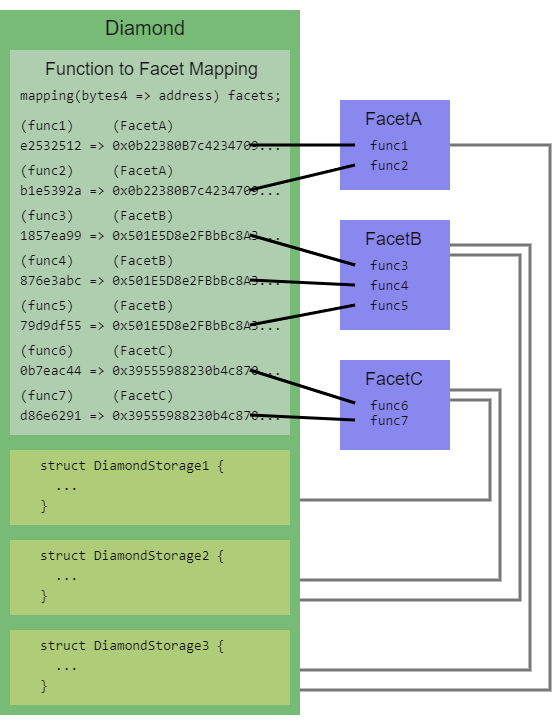
\includegraphics[scale=0.5]{diamond_struct.png}
  \centering 
  \label{fig:diamond_struct}
\end{figure}

% \begin{figure}[h]
  % \caption{Schéma représentatif des appels à un diamant.}
  % 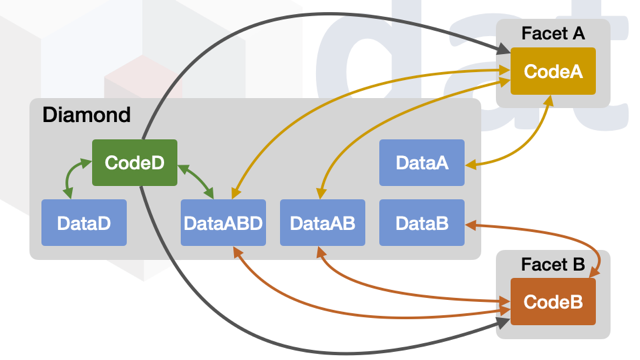
\includegraphics[scale=0.5]{diamond_ex.png}
  % \centering
  % \label{fig:diamond_ex}
% \end{figure}


\subsection{Comparaison de mon prototype et du diamant}

Il est évident que l'implémentation officielle est bien plus avancée que mon prototype,
néanmoins nous pouvons voir que mon prototype utilise la même technique que l'implémentation officielle.
La plus grande différence entre le diamant et mon prototype est la modularité. En effet, mon prototype étant
un prototype je ne me suis pas concentré sur la simplicité de l'interface d'utilisation. Mon objectif était 
de réaliser un "Proof of Concept". L'objectif est réalisé j'ai un prototype fonctionnel et cela m'a permis 
de bien mieux comprendre le fonctionnement de l'implémentation officielle. J'ai pu acquérir les connaissances
bas niveaux nécessaires à de telle utilisation.


\newpage
\section{Problèmes soulevés}

Pouvoir modifier dynamiquement le comportement d'un smart contract comporte des risques.
En effet, comme expliquer précédemment les utilisateurs ont confiance dans les smarts contracts
car, leurs comportements sont immuables. Il est donc primordial de trouver des solutions afin de garder
la confiance des utilisateurs. Pour cela il existe différentes type de méthode appelé gouvernance:

\subsection{Gouvernance avec un administrateur}

La première technique de gouvernance qui est aussi la plus simple est avec un administrateur.
En effet, à la création d'un smart contract on peut définir un administrateur qui à tout contrôle
sur le comportement du smart contract. Il peut ajouter, modifier ou supprimer du comportement.
Dans ce cas utiliser le smart contract revient à utiliser une alternative centralisée. On perd
l'avantage du décentralisé de la blockchain.

\subsection{Gouvernance avec un système de vote}

Un système de gouvernance avec un système de vote permet de garder l'aspect décentralisé d'un smart contract.
Dans ce type de système il est nécessaire définir un protocole de proposition et d'acceptation
d'un changement. Pour définir la valeur d'un vote on peut utiliser un smart contract implémentant un Token.
Un Token est défini dans l'environnement Ethereum par le la norme ERC-20. Cette norme définie qu'un Token
fongible (Un bien fongible est un bien qui se caractérise par son appartenance à un genre et non par 
une identité propre). Un Token peut donc s'apparenter à une monnaie. Un Token peut s'échanger ou être créé.

À la création d'un smart contract modifiable gouverné par un système de Vote, on peut imaginer générer une quantité
fixe de Token est les attribuer à un nombre restreint de parti prenante. Afin d'accepter une proposition on demande
aux personnes ayant des Tokens de voter. Le vote consiste à pour toutes les personnes ayant des Tokens de donner leurs
accord ou non accord (oui ou non) par rapport à une proposition. S'ils donnent leurs accords alors leur quantité 
de Token est ajouté au nombre de vote pour la proposition. Si le nombre de vote pour une proposition est supérieur ou
égal à la quantité totale * 0.8. Alors 80\% des personnes ayant le droit de vote sont d'accord pour la modification.
Le code permettant d'ajouter une proposition et de voter doit être immuable afin de protéger contre un vote
souhaitant modifier le système de vote.

Par exemple: deux entreprises créer un smart contract modifiable (basé sur la bibliothèque Diamond). À la création
elle génère 1000 Tokens (500 pour les deux entreprises). Afin d'ajouter, modifier ou supprimer 
du comportement au smart contract il est nécessaire d'obtenir l'accord de 80\% des tokens créer. 
L'entreprise 1 demande d'ajouter une fonctionnalité nommée "A". La proposition A reçoit directement le nombre de token
de l'entreprise 1 soit 500. Si l'entreprise 2 vote "oui" alors le total des votes sera de 1000 et vu que $1000 > 1000*0.8$
alors la proposition est accepté.

L'avantage de cette méthode est que l'on peut très facilement ajouter des acteurs.

Par exemple: L'entreprise 2 à un accord avec une nouvelle entreprise nommée "3". Cet accord consiste à obtenir
25\% des droits de vote sur le smart contract modifiable. Afin de réaliser cette action l'entreprise 2 envoi 250
token à l'entreprise 3.


Ce système permet une grande flexibilité est permet d'instaurer un vrai système démocratique au sein de la blockchain.
Cela permet de récupérer la confiance des utilisateurs car, toute modification doit être approuvé.

\subsection{Gouvernance avec un Multisig wallet}



\newpage
\section{Pedagogie}

Statut: À faire
\begin{itemize}
    \item Récapitulatif des réunions.
    \item Organisation du transfert de connaissance.
\end{itemize}

\subsection{Recapilulatif des réunions}

\subsection{Mon organisation}


\newpage
\section{Ouvertures}

Statut: À faire
\begin{itemize}
    \item Ajouter du type checking dans solidity
    \item Nouvel opcode ?
\end{itemize}

\subsection{Améliorer la manière de créer des contracts dynamiquement modifiable dans solidity}


\subsection{Ajout d'un système de type plus intelligent pour prévenir les erreurs}


\newpage
\section{Conclusion}

Ce projet m'a permis de découvrir un domaine qui m'intéresse vraiment, la blockchain. La blockchain est selon moi
le futur pour énormément d'applications centralisées. Et pouvoir travailler un mois à plein temps dessus m'a permis 
d'acquérir des compétences dans ce domaine prometteur. De plus, avoir été encadré par des chercheurs de l'INRIA 
m'a permis de découvrir est m'intéresser au monde de la recherche que je trouve passionnant. J'ai pu avec leurs
aides acquérir et comprendre l'état de l'art dans le domaine des smarts contract modifiable et j'en suis à la fois
fier et excité. Nous avons pu définir des idées d'améliorations qui permettraient de simplifier la vitesse d'adoption
de cette technologie en la rendant plus sûre et moins difficile d'utilisations à tous les développeurs. J'ai
envie de continuer ma vie dans ce domaine qui est la blockchain et je sais que ce TER m'a aidé à renforcer mes
connaissances. 

Ce fût une expérience humaine et qui malgré le contexte sanitaire difficile m'a permis de me rapprocher de mon 
professeur Dr Luigi Liquori qui m'a fait confiance et qui m'a mis en avant devant ses pairs chercheurs et doctorants.
J'espère après mon stage poursuivre mon travail dans ce domaine et j'espère pouvoir apporter quelque chose dans quelques
années à la communauté internationale. Après ce projet, je continuerai peut-être en thèse ou en entrepreneuriat. 

Je remercie Dr Luigi Liquori pour m'avoir fait confiance, je remercie aussi Dr Daniel Da Carvalho et Mr Mansur Khazeev
de m'avoir écouté et corriger mes travaux et je remercie toutes l'équipe pédagogique d'avoir pu me transformer en le 
futur diplômé que je serais très bientôt. 


\newpage
\begin{thebibliography}{9}

\bibitem{Bitcoin} 
Satoshi Nakamoto: Bitcoin white paper,
\\\url{https://bitcoin.org/bitcoin.pdf}

\bibitem{Ethereum} 
Vitalik Buterin: Ethereum white paper,
\\\url{https://ethereum.org/en/whitepaper/}

\bibitem{Tezos} 
L.M Goodman. Tezos white paper,
\\\url{https://tezos.com/}

\bibitem{OpenZeppelin} 
OpenZeppelin,
\\\url{https://docs.openzeppelin.com/openzeppelin/}

\bibitem{stateofart} 
The state of smarts contract Upgrades,
\\\url{https://blog.openzeppelin.com/the-state-of-smart-contract-upgrades/}

\bibitem{PROXY} 
Proxy: How to Write Upgradable Smart Contracts,
\\\url{https://simpleaswater.com/upgradable-smart-contracts/}


\bibitem{Truffle} 
Truffle suite: Sweet Tools for Smart Contracts,
\\\url{https://www.trufflesuite.com/}

\bibitem{Ganache}
Ganache: One Click Blockchain,
\\\url{https://www.trufflesuite.com/ganache/}


\bibitem{EIP}
Ethereum Improvement Proposals,
\\\url{https://eips.ethereum.org/}

\bibitem{OOPSLA} 
P. Di Gianantonio, F. Honsell and L. Liquori, "A Lambda Calculus of Objects with Self-Inflicted", Proceedings of OOPSLA. ACM Press, New York, p. 166–178, 1998.

\bibitem{INRIA-ACC}
Langages pour la définition de contrats intelligents  pour des blockchains autorisées et portefeuilles distribués, proposition de thèse Inria \& Accenture, 2019.

\end{thebibliography}




\end{document}

